\subsubsection{Khái niệm}
Thay vì đi tìm mô mô hình ước lượng tỷ lệ $P(Y =1)$ như trong mô hình logit. một hướng tiếp cận khác là đi tìm một siêu mặt phẳng có khả năng chia cắt không gian của bộ số liệu ra làm 2 phần. Nói cách khác là ước lượng một hàm:

$$
\large
f(x) = \beta_0 + \beta1 x_1 + \beta_2 x2 ...\beta_p x_p
$$

sao cho các quan sát thuộc 2 nhóm khác nhau sẽ được quyết định bằng dấu của $f(x)$, tức là nămg ở 2 phía của siêu mặt phẳng:

$$
\large
\beta_0 + \beta1 x_1 + \beta_2 x2 ...\beta_p x_p = 0
$$

Mô hình véc tơ máy hỗ trợ (Support Vector Machine - SVM) là một trong những mô hình thuộc loại này. SVM phát triển từ những năm 1990 và nhanh chóng được mọi người đón nhận vì khả năng phân loại tốt trong nhiều trường hợp khác nhau.

\paragraph{Phân loại lề cực đại (Maximal Marginal Classifier)}
Mô hình SVM được phát triển từ một phương pháp phân loại khá đơn giản gọi là phương pháp maximal margin classifier \parencite{boser1992training}. Thông thường, nếu như một bộ số liệu có thể được chia ra bởi một siêu mặt phẳng ngăn cách, chúng ta sẽ có thể tìm được vô siêu mặt phẳng như thế. Điều này là do các mặt phẳng có di chuyển nhẹ lên xuống hoặc quay mà không chạm tới các quan sát. Để xây dựng một mô hình phân loại dựa trên một siêu mặt phẳng phân loại,  chúng ta phải có một phương pháp hợp lý để chọn mặt phẳng hợp lý trong số vô số siêu mặt phẳng này.

Phương pháp Maximal Marginal Classifier lựa chọn siêu mặt phẳng mà nằm xa nhất các quan sát trong bộ số liệu. Nếu chúng ta tính khoảng cách từ các quan sát tới siêu mặt phẳng đã cho, khoảng cách nhỏ nhất từ các quan sát đến siêu mặt phẳng này gọi là lề (margin) của siêu mặt phẳng. Siêu mặt phẳng lề cực đại mà chúng ta chọn trong phương pháp này là siêu mặt phẳng mà lề là lớn nhất.

\begin{figure}
  \centering
   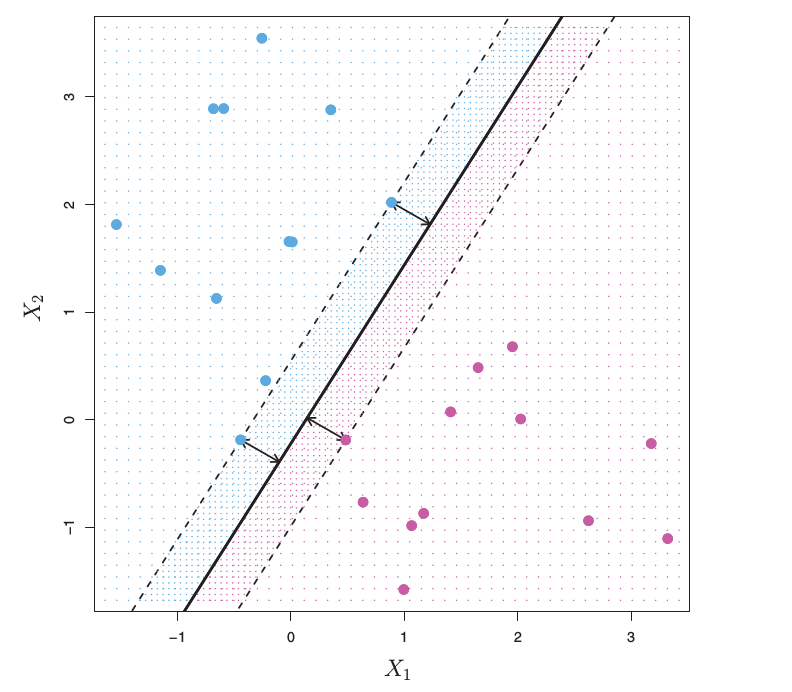
\includegraphics[width=0.5\textwidth]{./Figures/maxim_margin_example.png}
   \caption{Ví dụ về siêu mặt phẳng lề cực đại trong không gian 2 chiều.}
   \label{fig:maxim_margin_example}
\end{figure}

Siêu mặt phẳng được ước lượng bằng cách giải phương trình:


 $$
\large
\begin{cases}
\max\limits_{\beta_0, \beta_1,...,\beta_p}M\\

\sum_{j = 1}^p \beta_j^2 = 1\\

y_i(\beta_0 + \beta_1x_{i2} + ... + \beta_px_{ip}) \geq M \qquad \forall i = 1, 2, ...n
\end{cases}
$$

trong đó $M$ là độ rộng của lề, chúng ta tìm giá trị tối đa cho giá trị này, dưới ràng buộc rằng 
 $$
\large
y_i(\beta_0 + \beta_1x_{i2} + ... + \beta_px_{ip}) \geq M \qquad \forall i = 1, 2, ...n
$$
để đảm bảo rằng mỗi quan sát đều nằm trên đúng phía của siêu mặt phẳng phân loại, với điều kiện rằng $M$ không âm.
Khoảng cách từ quan sát thứ $i$ đến siêu mặt phẳng có thể được tính bằng: 

$$
y_i(\beta_0 + \beta_1x_{i2} + ... + \beta_px_{ip})
$$


\paragraph{Phương pháp phân loại hỗ trợ máy}

Phương pháp phân loại lề cực đại không thể thực hiện được trong trường hợp không tồn tại một siêu mặt phẳng nào có thể chia tách bộ số liệu ra thành 2 nhóm.

Một cải tiến của phương pháp này là phương pháp hỗ trợ máy, trong đó siêu mặt phẳng được ước lượng bằng phương trình:

$$
\large
\begin{cases}
\max\limits_{\beta_0, \beta_1,...,\beta_p, \epsilon_1, ... , \epsilon_n}M\\

\sum_{j = 1}^p \beta_j^2 = 1\\

y_i(\beta_0 + \beta_1x_{i2} + ... + \beta_px_{ip}) \geq M(1-\epsilon_i) \\

\epsilon_i \geq 0, \quad \sum_{i = 1}^n \epsilon_i \leq C
\end{cases}
$$

Trong đó $C$ là một tham số không âm do ta lựa chọn. $\epsilon_i$ là các hệ số không âm cho phép quan sát thứ $i$ vi phạm quy tắc của siêu mặt phẳng biên cực đại, với $C$ là giới hạn cho số sai phạm này. Nếu $0 < \epsilon_i < 1$, điểm $i$ nằm ở phía trong biên nhưng vẫn đúng phía của siêu mặt phẳng phân loại. Nếu $\epsilon_i = 1$, điểm $i$ nằm ở sai phía của siêu mặt phẳng phân loại.

\paragraph{Các kernel và mô hình véc tơ hỗ trợ máy}

Mô hình véc tơ hỗ trợ máy (Support Vector Machine) là một mở rộng của mô hình phân loại vectơ hỗ trợ, giúp xây dựng các mô hình phân loại phi tuyến. Mô hình này sử dụng một phép chiếu $\Phi$, chiếu các quan sát từ một không gian không phân biệt tuyến tính lên một chiều không gian mới mà ở đó các quan sát trở nên phân biệt tuyến tính.

Trong thực tế, việc thực hiện phép chiếu $\Phi$ này có thể trở nên rất khó khăn khi kích cỡ của bộ số liệu lớn. \textcite{scholkopf1999advances} chỉ ra rằng đối với một số phép chiếu, để ước lượng được mô hình véc tơ hỗ trợ, chúng ta chỉ cần tính được tích vô hướng của các quan sát trong bộ dữ liệu, thủ thuật này được gọi là thủ thuật kernel. Mô hình véc tơ hỗ trợ sử dụng thủ thuật kernel này được gọi là mô hình véc tơ hỗ trợ máy (SVM). Một cách tổng quát, mô hình SVM ước lượng:

$$
f(x) = \beta_0 + \sum\alpha_i K(x, x_i)
$$

trong đó $\beta0$, $\alpha_i$ là các hệ số cần ước lượng, $K(x, x_i)$ được gọi là hàm kernel, $x_i$ và $x$ lần lượt là véc tơ của quan sát thứ $i$ trong bộ số liệu và vectơ của quan sát mới cần phân loại.

Một số hàm kernel phổ biến được sử dụng rộng rãi là:

\begin{itemize}
  \item{$K(x, x_i) = x_i^T x$}: Hàm kernel tuyến tính, đây thực chất là hàm kernel của mô hình phân loại vec tơ hỗ trợ bình thường.
  \item{$K(x, x_i) =  (1 + \sum_{j = 1}^p x_i x)^d$}: Hàm kernel đa thức với tham số $d$ là bậc của đa thức ước lượng.
  \item{$K(x, x_i) = e^{-\sigma{\|x - x_i\|}^2}$}: Hàm kernel tròn với tham số $\sigma$ quyết định bán kính của đường tròn phân chia các quan sát
\end{itemize}

\begin{figure}
  \centering
    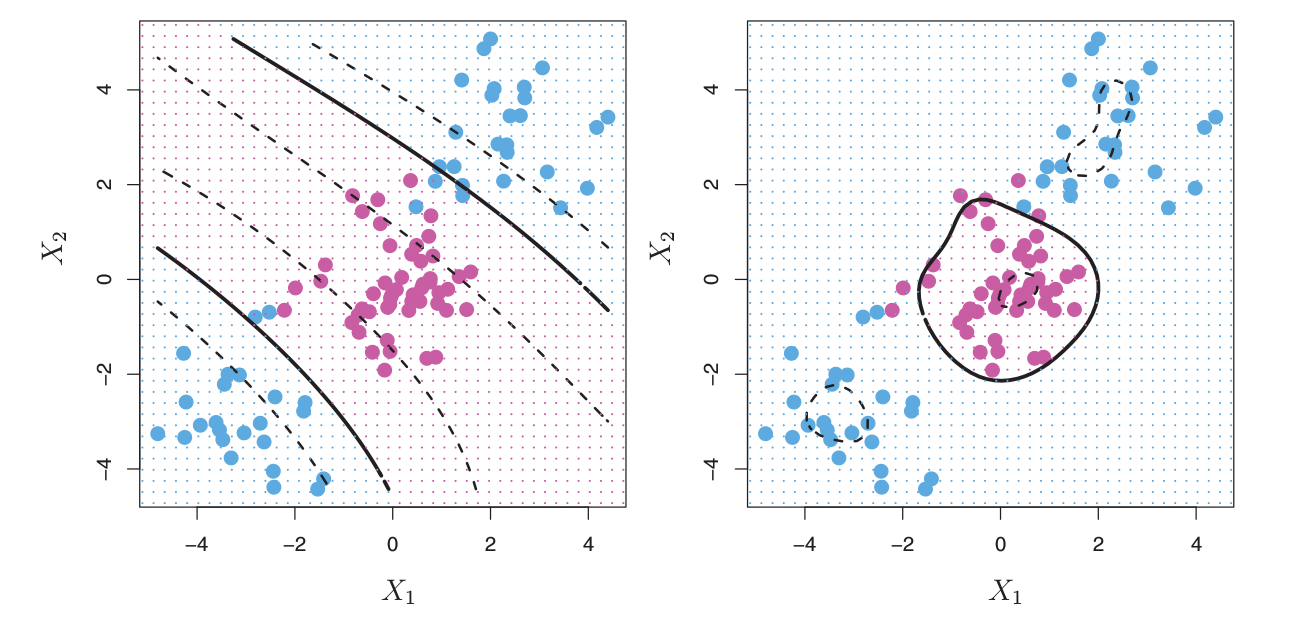
\includegraphics[width=\textwidth]{./Figures/svm_kernel_example.png}
  \caption[Ví dụ về phân loại sử dụng mô hình SVM]{Ví dụ về phân loại sử dụng mô hình SVM sử dụng kernel đa thức với d = 3 (trái) và kernel tròn (phải)}
  \label{fig:svm_kernel_example}
\end{figure}

\subsubsection{Quy trình xây dựng một mô hình véc tơ máy hỗ trợ}

Trong xây dựng một mô hình SVM, việc lựa chọn kernel thích hợp và việc điều chỉnh để có được tham số thích hợp cho kernel đó là yếu tố vô cùng quan trọng. 
\textcite{hsu2003practical} đưa ra một quy trình để có thể đạt được kết quả chấp nhận được đối với hầu hết các trường hợp. Quy trình đó như sau:

\begin{itemize}
  \item Thực hiện chuẩn hoá bộ số liệu
  \item Ưu tiên sử dụng kernel tròn (RBF): $K(x, x_i) = e^{-\sigma{\|x - x_i\|}^2}$
  \item Sử dụng kiểm định chéo để tìm tham số tốt nhất cho $C$ và $\sigma$.
  \item Sử dụng tham số $C$ và $\sigma$ tốt nhất ước lượng được để ước lượng trên toàn bộ bộ số liệu dùng để xây dựng mô hình.
  \item Kiểm tra hiệu quả mô hình.
\end{itemize}

Trong bài này ta sẽ đi theo quy trình này để xây dựng mô hình SVM, sử dụng phần mềm \texttt{LIBSVM} \textcite{CC01a}, một phần mềm phổ biến được sử dụng rộng rãi để xây dựng các mô hình SVM.
